\documentclass[tikz,border=4pt]{standalone}
\usepackage{amsmath,amssymb}
\usepackage[scaled=0.95]{helvet}
\renewcommand{\familydefault}{\sfdefault}
\usepackage{sfmath}
\usetikzlibrary{calc,arrows.meta}
\definecolor{cBlue}{RGB}{0,114,178}
\definecolor{cOrange}{RGB}{213,94,0}
\definecolor{cGreen}{RGB}{0,140,100}
\definecolor{cPurple}{RGB}{124,77,160}
\definecolor{cGray}{RGB}{110,110,110}
\definecolor{cNavy}{RGB}{24,40,68}
\hyphenpenalty=10000\exhyphenpenalty=10000
\begin{document}
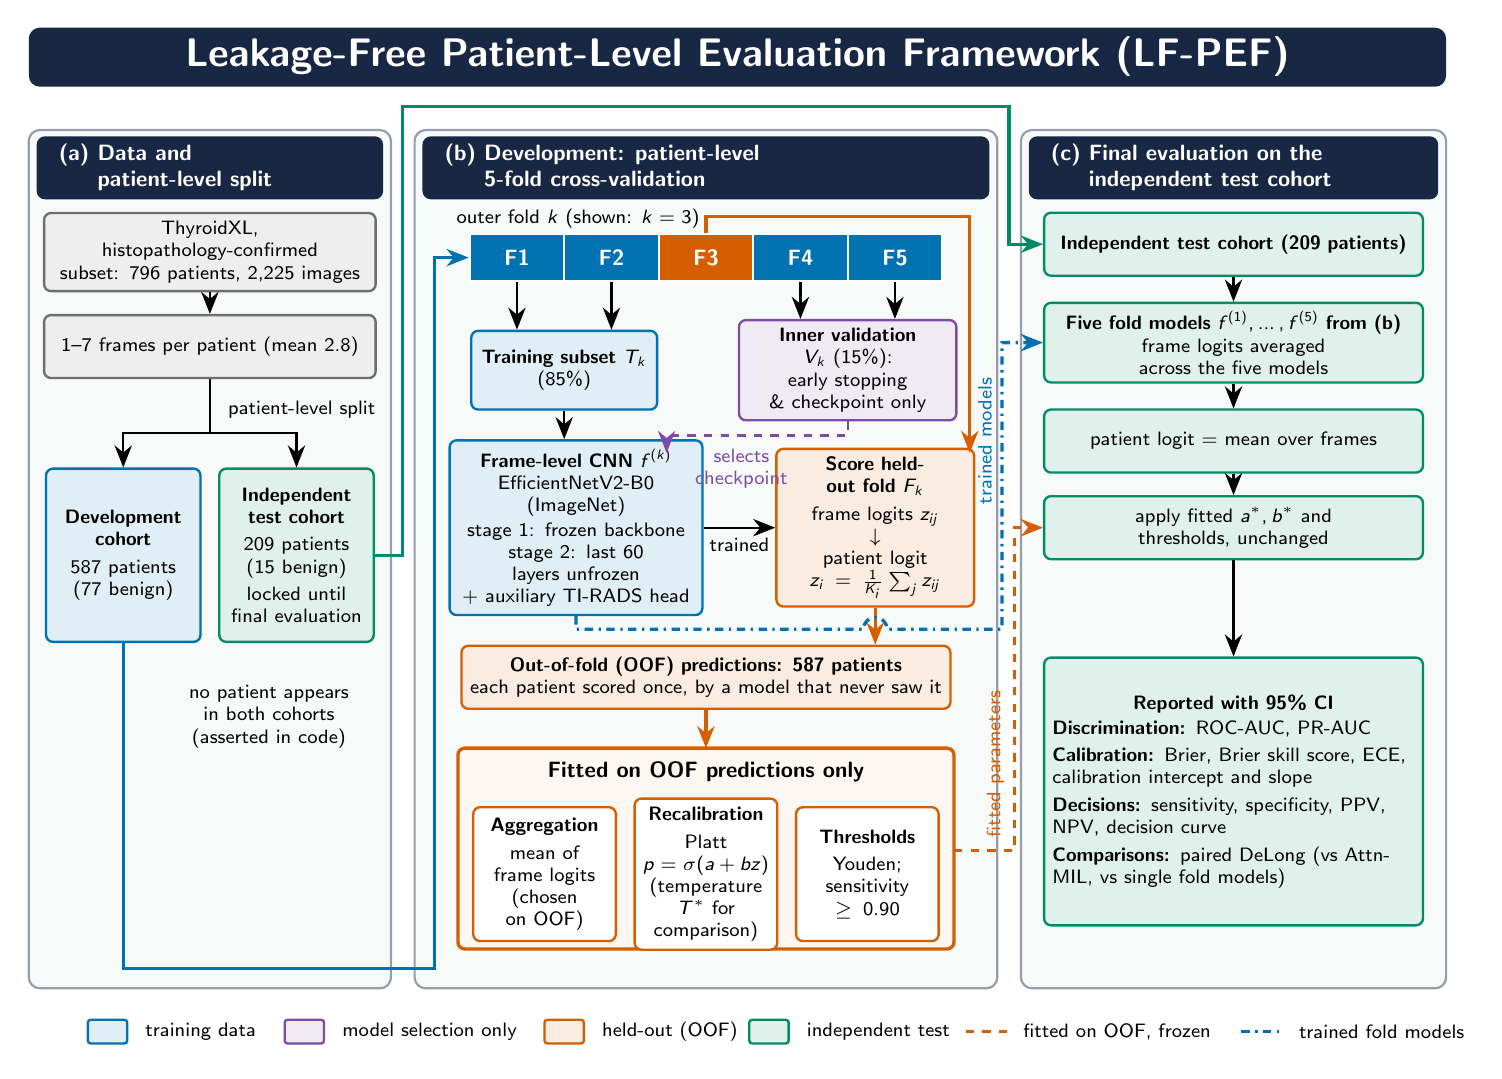
\begin{tikzpicture}[
  >={Stealth[length=2.8mm, width=2.2mm]}, line width=0.85pt,
  box/.style={draw=#1, fill=#1!12, rounded corners=2.5pt, align=center,
              font=\scriptsize, inner sep=3pt, minimum height=8mm},
  hdr/.style={font=\footnotesize\bfseries, align=left, anchor=west, text=white},
  hbar/.style={fill=cNavy, rounded corners=3pt},
  panel/.style={draw=cNavy!45, line width=0.8pt, rounded corners=4pt, fill=cNavy!3},
  fold/.style={draw=white, line width=0.8pt, minimum width=12mm, minimum height=6mm,
               font=\footnotesize\bfseries, text=white},
  lab/.style={font=\scriptsize, align=center}
]
% ---------------- panels & title ----------------
\draw[panel] (0,0.1) rectangle (4.6,11.0);
\draw[panel] (4.9,0.1) rectangle (12.3,11.0);
\draw[panel] (12.6,0.1) rectangle (18.0,11.0);
\fill[hbar] (0.1,10.12) rectangle (4.5,10.92);
\fill[hbar] (5.0,10.12) rectangle (12.2,10.92);
\fill[hbar] (12.7,10.12) rectangle (17.9,10.92);
\node[hdr] at (0.25,10.52)  {(a) Data and\\\phantom{(a) }patient-level split};
\node[hdr] at (5.15,10.52)  {(b) Development: patient-level\\\phantom{(b) }5-fold cross-validation};
\node[hdr] at (12.85,10.52) {(c) Final evaluation on the\\\phantom{(c) }independent test cohort};
\fill[cNavy, rounded corners=4pt] (0,11.55) rectangle (18.0,12.3);
\node[font=\Large\bfseries, text=white] at (9,11.93) {Leakage-Free Patient-Level Evaluation Framework (LF-PEF)};

% ---------------- panel (a) ----------------
\node[box=cGray, text width=4.0cm] (A1) at (2.3,9.45)
  {ThyroidXL, histopathology-confirmed\\subset: 796 patients, 2,225 images};
\node[box=cGray, text width=4.0cm] (A2) at (2.3,8.25) {1--7 frames per patient (mean 2.8)};
\draw[->] (A1) -- (A2);
\draw (A2.south) -- (2.3,7.15) coordinate (S);
\node[lab, anchor=west] at (2.4,7.45) {patient-level split};
\node[box=cBlue, text width=1.75cm, minimum height=22mm] (A3) at (1.2,5.6)
  {\textbf{Development cohort}\\[2pt]587 patients\\(77 benign)};
\node[box=cGreen, text width=1.75cm, minimum height=22mm] (A4) at (3.4,5.6)
  {\textbf{Independent test cohort}\\[2pt]209 patients\\(15 benign)\\[2pt]{\scriptsize locked until final evaluation}};
\draw[->] (S) -| (A3.north);
\draw[->] (S) -| (A4.north);
\node[lab, text width=2.5cm] at (3.05,3.55) {no patient appears in both cohorts (asserted in code)};

% ---------------- panel (b) ----------------
\foreach \i/\x/\c in {1/6.2/cBlue,2/7.4/cBlue,3/8.6/cOrange,4/9.8/cBlue,5/11.0/cBlue}
  \node[fold, fill=\c] (F\i) at (\x,9.38) {F\i};
\node[lab, anchor=west] at (5.3,9.88) {outer fold $k$ (shown: $k = 3$)};
\node[box=cBlue, text width=2.15cm, minimum height=10mm] (T) at (6.8,7.95) {\textbf{Training subset $T_k$}\\(85\%)};
\node[box=cPurple, text width=2.55cm, minimum height=10mm] (V) at (10.4,7.95) {\textbf{Inner validation}\\$V_k$ (15\%): early stopping\\\& checkpoint only};
\foreach \f/\t in {F1/T,F2/T,F4/V,F5/V} \draw[->] (\f.south) -- (\f.south |- \t.north);

\node[box=cBlue, text width=3.0cm, minimum height=19mm] (M) at (6.95,5.95)
  {\textbf{Frame-level CNN $f^{(k)}$}\\EfficientNetV2-B0\\(ImageNet)\\[1pt]{\scriptsize stage 1: frozen backbone\\stage 2: last 60 layers unfrozen\\+ auxiliary TI-RADS head}};
\node[box=cOrange, text width=2.3cm, minimum height=19mm] (S1) at (10.75,5.95)
  {\textbf{Score held-out fold $F_k$}\\[2pt]{\scriptsize frame logits $z_{ij}$\\$\downarrow$\\patient logit\\$z_i = \frac{1}{K_i}\sum_j z_{ij}$}};
\draw[->] (T.south) -- (T.south |- M.north);
\draw[->, cPurple, dashed] (V.south) -- (10.4,7.12) -- (8.1,7.12) -- (8.1,6.9);
\node[lab, text=cPurple, anchor=north] at (9.05,7.08) {selects\\checkpoint};
\draw[->, cOrange, line width=1.2pt] (F3.north) -- (8.6,9.9) -- (11.95,9.9) -- (11.95,6.9);
\draw[->] (M.east) -- node[lab, below]{trained} (S1.west);

\node[box=cOrange, text width=6.0cm] (O) at (8.6,4.05)
  {\textbf{Out-of-fold (OOF) predictions: 587 patients}\\{\scriptsize each patient scored once, by a model that never saw it}};
\draw[->, cOrange, line width=1.2pt] (S1.south) -- (S1.south |- O.north);

\draw[cOrange, line width=1.2pt, rounded corners=2.5pt, fill=cOrange!5] (5.45,0.6) rectangle (11.75,3.15);
\node[font=\footnotesize\bfseries] at (8.6,2.85) {Fitted on OOF predictions only};
\node[box=cOrange, fill=white, text width=1.6cm, minimum height=17mm] (P1) at (6.55,1.55) {\textbf{Aggregation}\\[2pt]{\scriptsize mean of frame logits\\(chosen on OOF)}};
\node[box=cOrange, fill=white, text width=1.6cm, minimum height=17mm] (P2) at (8.6,1.55) {\textbf{Recalibration}\\[2pt]{\scriptsize Platt\\$p=\sigma(a + b z)$\\(temperature $T^{*}$ for comparison)}};
\node[box=cOrange, fill=white, text width=1.6cm, minimum height=17mm] (P3) at (10.65,1.55) {\textbf{Thresholds}\\[2pt]{\scriptsize Youden;\\sensitivity $\geq 0.90$}};
\draw[->, cOrange, line width=1.2pt] (O.south) -- (8.6,3.15);

% ---------------- panel (c) ----------------
\node[box=cGreen, text width=4.6cm] (C1) at (15.3,9.55) {\textbf{Independent test cohort (209 patients)}};
\node[box=cGreen, text width=4.6cm, minimum height=10mm] (C2) at (15.3,8.3)
  {\textbf{Five fold models $f^{(1)},\dots,f^{(5)}$ from (b)}\\{\scriptsize frame logits averaged across the five models}};
\node[box=cGreen, text width=4.6cm] (C3) at (15.3,7.05) {patient logit $=$ mean over frames};
\node[box=cGreen, text width=4.6cm] (C4) at (15.3,5.95) {apply fitted $a^{*}, b^{*}$ and thresholds, unchanged};
\node[box=cGreen, text width=4.6cm, align=left, minimum height=34mm] (C5) at (15.3,2.6)
  {\centerline{\textbf{Reported with 95\% CI}}\\[1pt]
   {\scriptsize\textbf{Discrimination:} ROC-AUC, PR-AUC\\[2pt]
   \textbf{Calibration:} Brier, Brier skill score, ECE, calibration intercept and slope\\[2pt]
   \textbf{Decisions:} sensitivity, specificity, PPV, NPV, decision curve\\[2pt]
   \textbf{Comparisons:} paired DeLong (vs AttnMIL, vs single fold models)}};
\draw[->] (C1) -- (C2); \draw[->] (C2) -- (C3); \draw[->] (C3) -- (C4); \draw[->] (C4) -- (C5);

% ---------------- cross-panel connections ----------------
\draw[->, cBlue, line width=1.2pt] (A3.south) -- (1.2,0.35) -- (5.15,0.35) -- (5.15,9.38) -- (F1.west);
\draw[->, cGreen, line width=1.2pt] (A4.east) -- (4.75,5.6) -- (4.75,11.3) -- (12.45,11.3) -- (12.45,9.55) -- (C1.west);
\draw[->, dashed, cOrange, line width=1.2pt] (11.75,1.85) -- (12.52,1.85) -- (12.52,5.95) -- (C4.west);
\node[lab, text=cOrange, rotate=90, anchor=south] at (12.52,2.95) {fitted parameters};
% the five trained fold models are carried to the test branch (hop over the OOF arrow)
\draw[->, dash dot, cBlue, line width=1.2pt] (M.south) -- (6.95,4.66) -- (10.6,4.66) arc(180:0:0.15) -- (12.36,4.66) -- (12.36,8.3) -- (C2.west);
\node[lab, text=cBlue, rotate=90, anchor=south] at (12.36,7.05) {trained models};

% ---------------- legend ----------------
\begin{scope}[shift={(1.0,-0.45)}, font=\scriptsize]
  \foreach \c/\t/\x in {cBlue/training data/0, cPurple/model selection only/2.5, cOrange/held-out (OOF)/5.8, cGreen/independent test/8.4}{
    \node[draw=\c, fill=\c!12, minimum width=5mm, minimum height=3mm, rounded corners=1pt] at (\x,0) {};
    \node[anchor=west] at (\x+0.35,0) {\t};}
  \draw[dashed, cOrange, line width=1.2pt] (10.9,0) -- (11.45,0);
  \node[anchor=west] at (11.5,0) {fitted on OOF, frozen};
  \draw[dash dot, cBlue, line width=1.2pt] (14.4,0) -- (14.95,0);
  \node[anchor=west] at (15.0,0) {trained fold models};
\end{scope}
\end{tikzpicture}
\end{document}
